\documentclass[bachelor,ngerman,english]{GAUBM}

%  =================================================================================  %
%  ==========  PACKAGES  ===========================================================  %
%  =================================================================================  %
\usepackage[T1]{fontenc}
\usepackage[latin1]{inputenc}
\usepackage{babel}
\usepackage{amsmath}
\usepackage{amssymb} 
\usepackage{amsfonts}
\usepackage{bm}
\usepackage{lmodern}
\usepackage{calc}
\usepackage{float}
\usepackage{setspace}

\usepackage{svg}
\usepackage{graphicx}
\usepackage{xcolor}
\usepackage{subfigure}
\usepackage{floatflt}
\usepackage[it, bf]{caption}
\graphicspath{{./}{./figures/}{./logos/}}

\newcommand{\tabheadfont}[1]{\textbf{#1}}
\usepackage{colortbl}
\usepackage{booktabs}
\usepackage{longtable}
\usepackage{array}
\usepackage{hhline}

\usepackage{textcomp}
\usepackage{gensymb}
\usepackage{units} 

\usepackage[comma,numbers,sort&compress]{natbib}
\bibliographystyle{bthesis_raschke}
% \bibliographystyle{plainnat}

\usepackage{blindtext}
\usepackage{xspace}
\usepackage[pdfstartview=FitH, 
            breaklinks=true,
            bookmarksopen=true,
            bookmarksnumbered=true 
]{hyperref}


%  =================================================================================  %
%  ==========  PAGE SETUP  =========================================================  %
%  =================================================================================  %
\pagestyle{headings}

\setlength{\oddsidemargin}{0cm}
\setlength{\evensidemargin}{0cm}
\setlength{\topmargin}{-1cm}
\setlength{\textheight}{23cm}
\setlength{\textwidth}{16cm}

\renewcommand{\sectfont}{\bfseries\rmfamily}
\renewcommand{\floatpagefraction}{0.7}
\renewcommand{\textfraction}{0.1}


%  =================================================================================  %
%  ==========  COLOURS  ============================================================  %
%  =================================================================================  %
\definecolor{highlight}{RGB}{200, 210, 215}


%  =================================================================================  %
%  ==========  TABLES  =============================================================  %
%  =================================================================================  %
\newcolumntype{L}[1]{>{\raggedright\arraybackslash}p{#1}}
\newcolumntype{C}[1]{>{\centering\arraybackslash}p{#1}}
\newcolumntype{R}[1]{>{\raggedleft\arraybackslash}p{#1}}
\newcolumntype{?}{!{\vrule width .1mm}}
\newcolumntype{V}{!{\vrule width .3mm}}


%  =================================================================================  %
%  ==========  Patches  ============================================================  %
%  =================================================================================  %
\makeatletter
\g@addto@macro\bfseries{\boldmath} %Patch math in Section/Capter title
\makeatother
\input{style}
\begin{document}
	
\ThesisAuthor{Ireas Tom}{Raschke}
\PlaceOfBirth{Finsterwalde}
\ThesisTitle{\ttHWW Rekonstruktion mit Neutrino Gewichtung \& SPANet}{\ttHWW event reconstruction techniques using neutrino-weighting \& SPANet}
\FirstReferee{Prof.~Dr.~Arnulf Quadt}
\Institute{II. Physikalisches Institut}
\ReferenceNumber{M.Phy.408: Research Lab Course in Nuclear and Particle Physics}
\ThesisBegin{03}{11}{2023}
\ThesisEnd{03}{10}{2024}

\frontmatter
\maketitle
\cleardoublepage
\onehalfspacing
\tableofcontents
\mainmatter

\chapter{Introduction}
\label{ch:introduction}
As far back as 400 BC, humans pondered the fundamental makeup of the natural world. The Greek philosopher Democritus proposed the notion that matter cannot be infinitely divisible. Thus, there must exist a smallest, indivisible particle, which he termed the 'atom' (from Greek \textit{atomos} meaning 'indivisible'). Although this idea was not empirically tested but derived from philosophical musings, it marked the inception of the quest for a fundamental understanding of the universe.

More than 2000 years later, in 1808, the chemist John Dalton refined Democritus's idea by introducing the concept of elements. Each element was seen as a distinct, indivisible atom differing in mass and size. This refined model enabled Dalton to account for the apparent conservation of mass.

In the late 19$^\text{th}$ century, physicist Sir Joseph John Thomson developed an atomic model portraying atoms as positively charged spheres containing lighter, negatively charged particles known as electrons. The atom as a concept was no longer the smallest, most fundamental particle. Thomson's model was derived from experiments utilising a hot, radiating cathode emitting electrons, thus explaining the observed cathode electron beam.

In 1911, Ernest Rutherford conducted an experiment using an $\alpha$-particle beam directed at a thin gold foil. The results suggested that the majority of an atom's mass is concentrated in a very small volume – the positively charged nucleus – surrounded by negatively charged electrons orbiting in mostly empty space.

Two years later, in 1913, Niels Bohr refined the model further, likening the motion of electrons around the nucleus to planets orbiting the sun. He proposed that electrons move in circular orbits without emitting radiation, with orbit radii restricted to specific quantised values, marking the inception of quantum mechanics.

Electrons can transition between orbits by emitting or absorbing photons of quantised energies, thus explaining the photoelectric effect. In 1916, Arnold Sommerfeld expanded the Bohr model, permitting elliptical orbits and providing an explanation for the presence of closely spaced spectral lines.

In 1926, Werner Heisenberg and Erwin Schrödinger independently developed a mathematical framework for quantum mechanics. The requirement that electrons adhere to Schrödinger's equation led to the concept of atomic orbitals – regions in space with a high probability of containing electrons, subject to specific selection rules.

While the concept of an atomic nucleus was first proposed by Rutherford, it was initially thought to consist solely of positively charged protons. However, this model was expanded in 1932 by James Chadwick, who introduced neutral particles, neutrons, as constituents of the nucleus.

Today, research into the fundamental structure of nature continues, with particle physics superseding nuclear physics. The contemporary aim of particle physics is to develop a comprehensive understanding of fundamental phenomena, centred around formulating and expanding upon the Standard Model of particle physics, which stands as the most successful description of the fundamental nature of the universe.


\chapter{The Standard Model of Particle Physics}
\label{ch:standard_model}

The Standard Model of particle physics (SM) stands as the most triumphant framework to date in understanding the fundamental particles and their interactions. It encompasses all known elementary particles along with their antiparticles, and three out of the four recognised fundamental forces: the strong, weak, and electromagnetic forces. Notably, gravity remains beyond the scope of the SM.

The SM is a renormalisable quantum field theory characterised by an internal SU(3)$\otimes$SU(2)$\otimes$U(1) gauge symmetry. The SU(3) group symmetry elucidates the strong interactions, stemming from quantum chromodynamics (QCD) \cite{qcd}, while the SU(2)$\otimes$U(1) group symmetry corresponds to the electroweak interactions. The latter entails the unification of the electromagnetic force, originating from quantum electrodynamics (QED) \cite{qed01, qed02, qed03}, and the weak force, stemming from quantum flavour dynamics (QFD) \cite{qft}.

Incorporated into the electroweak interaction in 1967, the Brout-Englert-Higgs mechanism introduces a quantum Higgs-field \cite{higgs_mechanism_1, higgs_mechanism_2, higgs_mechanism_3}. This mechanism instigates spontaneous symmetry breaking within the SU(2)$\otimes$U(1) symmetry. Initially, all bosons are massless, yet this symmetry breaking results in bosons interacting with the Higgs-field to become massive. Fermions, too, acquire their masses via interaction with the Higgs-field. The massive gauge bosons of the electroweak interaction are denoted as the \zwboson. Furthermore, one of the degrees of freedom introduced by the Higgs-field which is not defined via the Brout-Englert-Higgs mechanism, manifests as the scalar Higgs-boson $H$ \cite{higgs_mechanism_1}.

Despite the SM's commendable precision in predicting most observations, certain phenomena elude its fundamental explanations. Notably, neutrino oscillations \cite{neutrino_oscillation} exemplify this shortfall, delineating flavour-changing neutrinos. This oscillation necessitates at least two massive neutrinos, while the SM posits all neutrinos as massless. Consequently, the SM fails to account for neutrino oscillations. Another enigma is dark matter \cite{dark_matter}. The measured rotational velocities of vast spiral galaxies necessitate significantly more mass than visible matter provides. These astronomical observations indicate the presence of a stable form of matter that eludes electromagnetic interaction, rendering it invisible. No particle within the SM can explain these measurements.


\section{Characteristics of the Top Quark}
\label{sec:theory_top}
The discovery of the top ($t$) quark took place in 1995 at \fermilab through the collaborative efforts of the \dzero \cite{top_production01} and \cdf \cite{top_production02} experiments. With a mass of $m_t=172.76\pm0.30,\text{GeV}$ \cite{top_mass}, the top quark is acknowledged as the most massive among all known quarks. Its exceedingly brief lifespan is approximately $tau_t\approx5\cdot10^{-25},\text{s}$ \cite{top_mass}. Upon decaying through the weak interaction, the top quark decays into a \wboson and a down-type quark which then undergoes hadronisation. The likelihood of decaying into a specific down-type quark is determined by the corresponding CKM-matrix element \cite{ckm_matrix}. Given that the CKM-matrix predominantly features vanishing off-diagonal elements, the primary decay mode for top quarks involves transitioning into \bquarks. Subsequently, the \wboson undergoes further decay, either into a charged lepton and neutrino, yielding one observable jet originating from the \bquark alongside a detectable lepton, or into a quark-antiquark pair, resulting in the production of three detectable jets.

Generating \tquarks necessitates significant energies owing to the mass of the \tquark. Such energies are attainable in hadron colliders. Figure~\ref{fig:production_ttz_ttw} illustrates two exemplar processes for \tquark production within \ttbar processes. Each of the two \tquarks decays as previously described. Thus, the observed signal is contingent upon the decay mode of the \wboson.


\section{Effective Field Theory}
\label{sec:theory_eft}
For examining phenomena beyond the Standard Model, one can adopt an Effective Field Theory (EFT) framework like the Standard-Model Effective Field Theory (SM-EFT) \cite{eft_operatorlist}. This approach assumes that the current Standard Model serves as a practical low-energy approximation, valid for interactions up to an energy scale $\Lambda$. It can be expanded using higher-dimensional interactions \cite{eft_introduction}. The transition to the Standard Model occurs through the decoupling of heavy particles at energies greater than $\Lambda$. Thus, higher-dimensional operators $Q$, suppressed by powers of $\Lambda$, are utilised in a perturbation expansion \cite{eft_introduction}.

\begin{align}
\mathcal{L}\text{SM-EFT} = \mathcal{L}\text{SM} + \frac{1}{\Lambda}\sum_{k}C_k^{(5)}Q_k^{(5)} + \frac{1}{\Lambda^2}\sum_{k}C_k^{(6)}Q_k^{(6)} + \mathcal{O}\left(\frac{1}{\Lambda^3}\right);.\label{eq:SM-EFT}
\end{align}

In this expansion, $\mathcal{L}_\text{SM}$ denotes the standard SM Lagrangian, $Q_k^{(n)}$ represents the $n$-dimensional interaction operators, and $C_k^{(n)}$ are their corresponding Wilson coefficients.

For a deeper understanding of \ttbarZ and \ttbarW production, it's valuable to scrutinise their pertinent operators. Given that the \zboson combines the $W^0$ and $B$ bosons originating from the Brout-Englert-Higgs mechanism, the operator %\optZ for the $tZ$ coupling is expressed as \cite{higgs_mechanism_1}

\begin{align}
Q_\text{tZ} &= \cos(\Theta_W)Q_\text{tW} - \sin(\Theta_W)Q_\text{tB};.\label{eq:OparatortZ}
\end{align}

Therefore, the operators for the $tW$ and the $tB$ couplings, along with their complex coefficients %\ctW and \ctB, are particularly pertinent for this analysis \cite{eft_operatorlist}. To quantify sensitivity, the separation power

\begin{align}
S &= \frac{1}{2}\sum_\text{Bins}\frac{\left(\text{EFT}_i-\text{SM}_i\right)^2}{\text{EFT}_i+\text{SM}_i}\label{eq:SeparationPower}
\end{align}

is employed. The expression within the summation is computed for each bin based on a given normalised distribution. Here, $\text{SM}$ denotes the Standard Model prediction, and $\text{EFT}$ incorporates a specific variation on one or multiple Wilson coefficients as shown in Equation~\ref{eq:SM-EFT}. Investigations concerning the sensitivity of various variables for these coefficients are summarised in Chapter~\ref{ch:eft_sensitivity}.


\chapter{Experimental Setup}
\label{ch:experimental_setup}
To collect data on \ttbarZ and \ttbarW events, a high-energy particle collider is indispensable. Additionally, a setup for signal detection and suitable reconstruction algorithms are required.

The Large Hadron Collider (\lhc), spanning 27 kilometres, operates as a proton-proton collider. During Run~I, it achieved a centre-of-mass energy of approximately 7-8 TeV, rising to 13 TeV in Run~II \cite{lhc2}. For Run~III, an anticipated centre-of-mass energy of 13.6 TeV is projected \cite{lhc_run3}. These high-energy collisions yield multiple particles, including \tquarks, which subsequently decay into additional particles. Detecting these events necessitates a calibrated detector system capable of measuring particle properties such as charge, momentum, and energy. Moreover, event reconstruction from measured signals involves employing various algorithms to reconstruct, for instance, particle trajectories and collision vertices.

The \atlas-detector \cite{atlas} serves as a versatile particle detector comprising distinct layers designed to detect various particles. These layers are arranged in concentric cylinders around the beam axis. Through tracking measurements and energy deposition of decay products, the initial particles can be reconstructed. Figure~\ref{fig:atlas} illustrates a schematic representation of these detector layers. Each layer is described below.

% \begin{figure}[t]
%     \centering
%     \includegraphics[width=.61\textwidth]{figures/atlas/atlas3.png}
%     \caption{Cross-section of the concentric layers within the \atlas Detector (\copyright{} \cern)}
%     \label{fig:atlas}
% \end{figure}

\section*{The Inner Detector}
The Inner Detector is tasked with precisely measuring the tracks of various charged particles. A 2 T magnetic field, generated by a central solenoid, causes the movement of charged particles to deflect via the Lorentz force. By measuring the curvature, precise momentum measurements and particle track reconstruction are achieved. This tracking system is vital for $b$-tagging, enabling the identification of secondary vertices, indicative of $b$-jets \cite{atlas}. Given the high particle density near the collision point, high-precision measurements utilise Pixel, Strip, and Transition Radiation Trackers.

The Pixel Tracker, constructed from silicon to withstand collision radiation, detects tracks near the collision point using small Pixel-modules \cite{atlas}. The Semiconductor Strip Tracker (SCT) comprises longer strips, enhancing tracking with larger scale measurements.

The Transition Radiation Tracker (TRT) consists of thin polyimide straws filled with a gas mixture \cite{atlas}. While offering a lower resolution, these straws provide a cost-effective means to cover a larger volume, contributing to precise measurements. The TRT aids in distinguishing electrons $e^\pm$ from charged pions $\pi^\pm$.

\section*{The Calorimeters}
As depicted in Figure~\ref{fig:atlas}, the calorimeters envelop the Inner Detector and the solenoid magnet. Generally, they measure particle energy by halting their motion. The \atlas-detector utilises electromagnetic and hadronic calorimeters, both sampling calorimeters comprising an absorber material inducing particle showers and an active medium for signal measurement \cite{atlas_calorimeter}.

The electromagnetic calorimeter detects particles interacting electromagnetically, with charged particles and photons generating electromagnetic showers. This facilitates reconstruction of initial particles, offering precise energy measurement and deposition location. Constructed with Lead as the absorber and liquid Argon as the active medium, it provides accurate measurements \cite{atlas_calorimeter}.

The hadronic calorimeter absorbs particles passing through the electromagnetic calorimeter that interact via the strong force. Hadronic showers produced may yield additional electromagnetic sub-showers, complicating reconstruction and reducing precision. Comprising steel as the absorber and plastic scintillating tiles, it fulfils its role effectively \cite{atlas_calorimeter}.

\section*{The Muon Spectrometer}
Serving as the outermost layer, the Muon Spectrometer employs a similar approach to the Inner Detector to measure muon momentum, typically undetected by the Inner Detector and Calorimeter. It comprises four subsystems \cite{atlas}.

For muon triggering and coordinate measurement, Resistive Plate Chambers (RPC) and Thin Gap Chambers (TGC) are deployed across different detector regions. Additionally, Cathode Strip Chambers (CSC) offer precise coordinate measurements at the detector ends. Monitored Drift Tubes (MDT) track muon trajectories' curvature. Outer toroidal magnets generate the magnetic field responsible for muon deflection \cite{atlas}.

\chapter{Methods}
\label{ch:methods}
\section{SPANet}
\section{Neutrino Weighting}

\chapter{Current Status}
\label{ch:current_status}

\chapter{Outlook}
\label{ch:outlook}

\section{ttH}


% \cleardoublepage
% \chapter{Introduction}
% As early as 400 BC, people were philosophising about the fundamentals of nature. The oldest known idea was formulated by the Greek philosopher Democritus, who postulated that matter can not be infinitely divisible. Thus, there has to be a smallest, indivisible particle which would be called atom (from Greek \textit{atomos}=indivisible). This idea was not experimentally tested but built purely on philosophical thoughts, however, it represents the begin of the search for a fundamental description of the universe.

% Over 2000 years later, in 1808, the chemist John Dalton refines the idea of Democritus by introducing the concept of elements. Each element has a unique indivisible atom and the different atoms differ in their mass and size. This refined model allowed Dalton to explain the apparent conservation of mass.

% In the late 19th century, in 1897, the physicist Sir Joseph John Thomson developed the Thomson-model. This atomic model describes atoms as positive charged spheres which contain lighter negative charged particles, so called electrons. The entire atom is electrically neutral to the outside. The atom itself was not the smallest, most fundamental particle any more. This model was built on the experiments using a hot, radiating cathode that emits electrons. Hence, the Thomson-model explained the observed cathode electron beam.

% In 1911, Ernest Rutherford conducted the famous Rutherford-experiment, which used an $\alpha$-particle beam that was focused onto a thin gold foil. The results of the experiments suggest that most of the mass in an atom is contained in a very small volume which is the positively charged atom nucleus. Almost the whole atom consist of empty space. The negatively charged electrons orbit the atom nucleus.

% Two years later, in 1913, Niels Bohr formulated another atomic model that described the movement of electrons around the nucleus like planets around the sun. He postulated that electrons move on circular orbits without emitting radiation. Additionally, the radii of those orbits can only be certain quantised values. Electrons are able to change their orbits by emitting or absorbing photons of certain energies. This model made it possible to explain the photoelectric effect. In 1916, the Bohr-model was expanded by Arnold Sommerfeld who generalised the electron orbits and allowed an elliptical shape. Thus, the Bohr-Sommerfeld-model explained, why there are multiple spectral lines very close to each other.

% In 1926, the physicist Werner Heisenberg and Erwin Schr�dinger both developed a mathematical description of quantum mechanics. Requiring that electrons fulfil the quantum mechanical Schr�dinger equation lead to the atomic-orbital-model. The orbits are space regions with high probability of containing electrons and they are classified by four quantum numbers. Additionally, those orbits must obey specific selection rules. 

% While the concept of an atomic nucleus was first formulated by Rutherford, it was first thought to only be made up of positively charged protons. However, this model was expanded in 1932 by James Chadwick, who introduced neutral charged particles, neutrons, that are also part of the atomic nucleus.  

% In 1968, deep inelastic scattering allowed scientist to analyse these nucleons further. Protons and neutrons are made up of even smaller particles which were called partons. Later they were identified as quarks. The quark particles were already proposed in 1964 by Murray Gell-Mann and George Zweig. Today, these quarks are part of the Standard Model of particle physics which is the most successful description of the fundamental nature of the universe.

% Modern particle physics' task is to find a general description of fundamental phenomena. It focuses on expanding and refining the Standard Model to find a unified theory. To find new physics beyond the Standard Model, different experiments test various predictions of the Standard Model.


% \chapter{The Standard Model of Particle Physics}
% The Standard Model of particle physics (SM) is the most successful description of the fundamental particles and their interactions to this day. It covers all known elementary particles and their antiparticles as well as three of the four known fundamental forces: the strong, weak and electromagnetic force. Gravity is not described in the SM. 

% The SM is a renormalisable quantum field theory which is defined by an internal SU(3)$\otimes$SU(2)$\otimes$U(1) gauge symmetry. The SU(3) group symmetry describes the strong interactions, originating from quantum chromodynamics (QCD) \cite{qcd}, and the SU(2)$\otimes$U(1) group symmetry corresponds to the electroweak interactions \cite{qed01, qed02, qed03}. The later being the unification of the electromagnetic force, originating from quantum electrodynamics (QED), and the weak force, originating from quantum flavour dynamics (QFD).

% In 1967, the Higgs mechanism was incorporated into the electroweak interaction \cite{higgs_mechanism_1, higgs_mechanism_2, higgs_mechanism_3}. The Higgs mechanism adds a Higgs quantum field that induces a spontaneous symmetry breaking in the SU(2)$\otimes$U(1) symmetry. Initially all bosons were massless, but this symmetry breaking causes all bosons interacting with the Higgs-field to become massive. Fermions also obtain their masses by interacting with the Higgs field. The massive gauge bosons of the electroweak interaction are known as the \zwboson. Additionally, one of the degrees of freedom introduced by the Higgs-field is not needed by the Higgs-mechanism, thus becoming the scalar Higgs-boson $H$ \cite{higgs_mechanism_1}.

% However, there are observed phenomena which cannot be explained using the SM. An example for this is neutrino oscillations \cite{neutrino_oscillation}, which describes flavour changing neutrinos. This oscillation requires neutrinos to have a mass difference but the SM predicts all neutrinos to be massless. Hence, the SM cannot explain the neutrinos oscillation. Another example is dark matter \cite{dark_matter}. Astronomical observation give evidence of a stable form that does not interact electromagnetically, making it invisible to current observations. The measured rotational velocity for large spiral galaxies requires a much larger mass than the visible matter provides.

% \section{Elementary Particles}
% The elementary particles are divided into fermions and bosons. Fermions have half-integer spin and make up matter, while bosons have integer spin and are responsible for mediating the strong, weak and electromagnetic force. All these particles also have an antiparticle partner, which has the same mass but opposite electric charge.

% Figure $\ref{fig:standard_model}$ shows the different SM-particles. Furthermore, it shows that fermions are subdivided into quarks and leptons, which both are divided into three generations. Particles corresponding to a higher generation have significantly increased masses.

% The six quarks are split into three up-type (up, charm, top) and three down-type (down, strange, bottom) quarks. The up-type quarks have an electric charge of $q_\text{up}=+\frac{2}{3}\,e$ and down-type quarks of $q_\text{down}=-\frac{1}{3}\,e$. All quarks also have a colour charge, thus participating in strong interactions. Fermions also have a weak isospin $T$ which is related to the electric charge $q$ and is a quantum number referring to the weak interactions \cite{qed03}. The third component of the weak isospin $T_3$ is conserved by weak interactions.

% Left-handed fermions, and quarks in particular, have a weak isospin of $T=\frac{1}{2}$, which can be grouped into doublets with $T_3=\pm\frac{1}{2}$. The positive sign corresponds to up-type quarks and the negative sign to down-type quarks, respectively. Right-handed fermions form singlets and the charged electroweak \wboson does not interact with them.

% Leptons on the other hand are split into charged leptons ($e, \mu, \tau$) and their corresponding neutrinos ($\nu_e, \nu_\mu, \nu_\tau$). The charged leptons all have an electric charge $q_\text{l}=-1\,e$, while neutrinos are electrically neutral. Left-handed leptons can also be grouped into doublets with $T_3=\pm\frac{1}{2}$, where neutrinos are the up-type particles and charged leptons the down-type.

% \begin{figure}[ht]
% 	\centering
% 	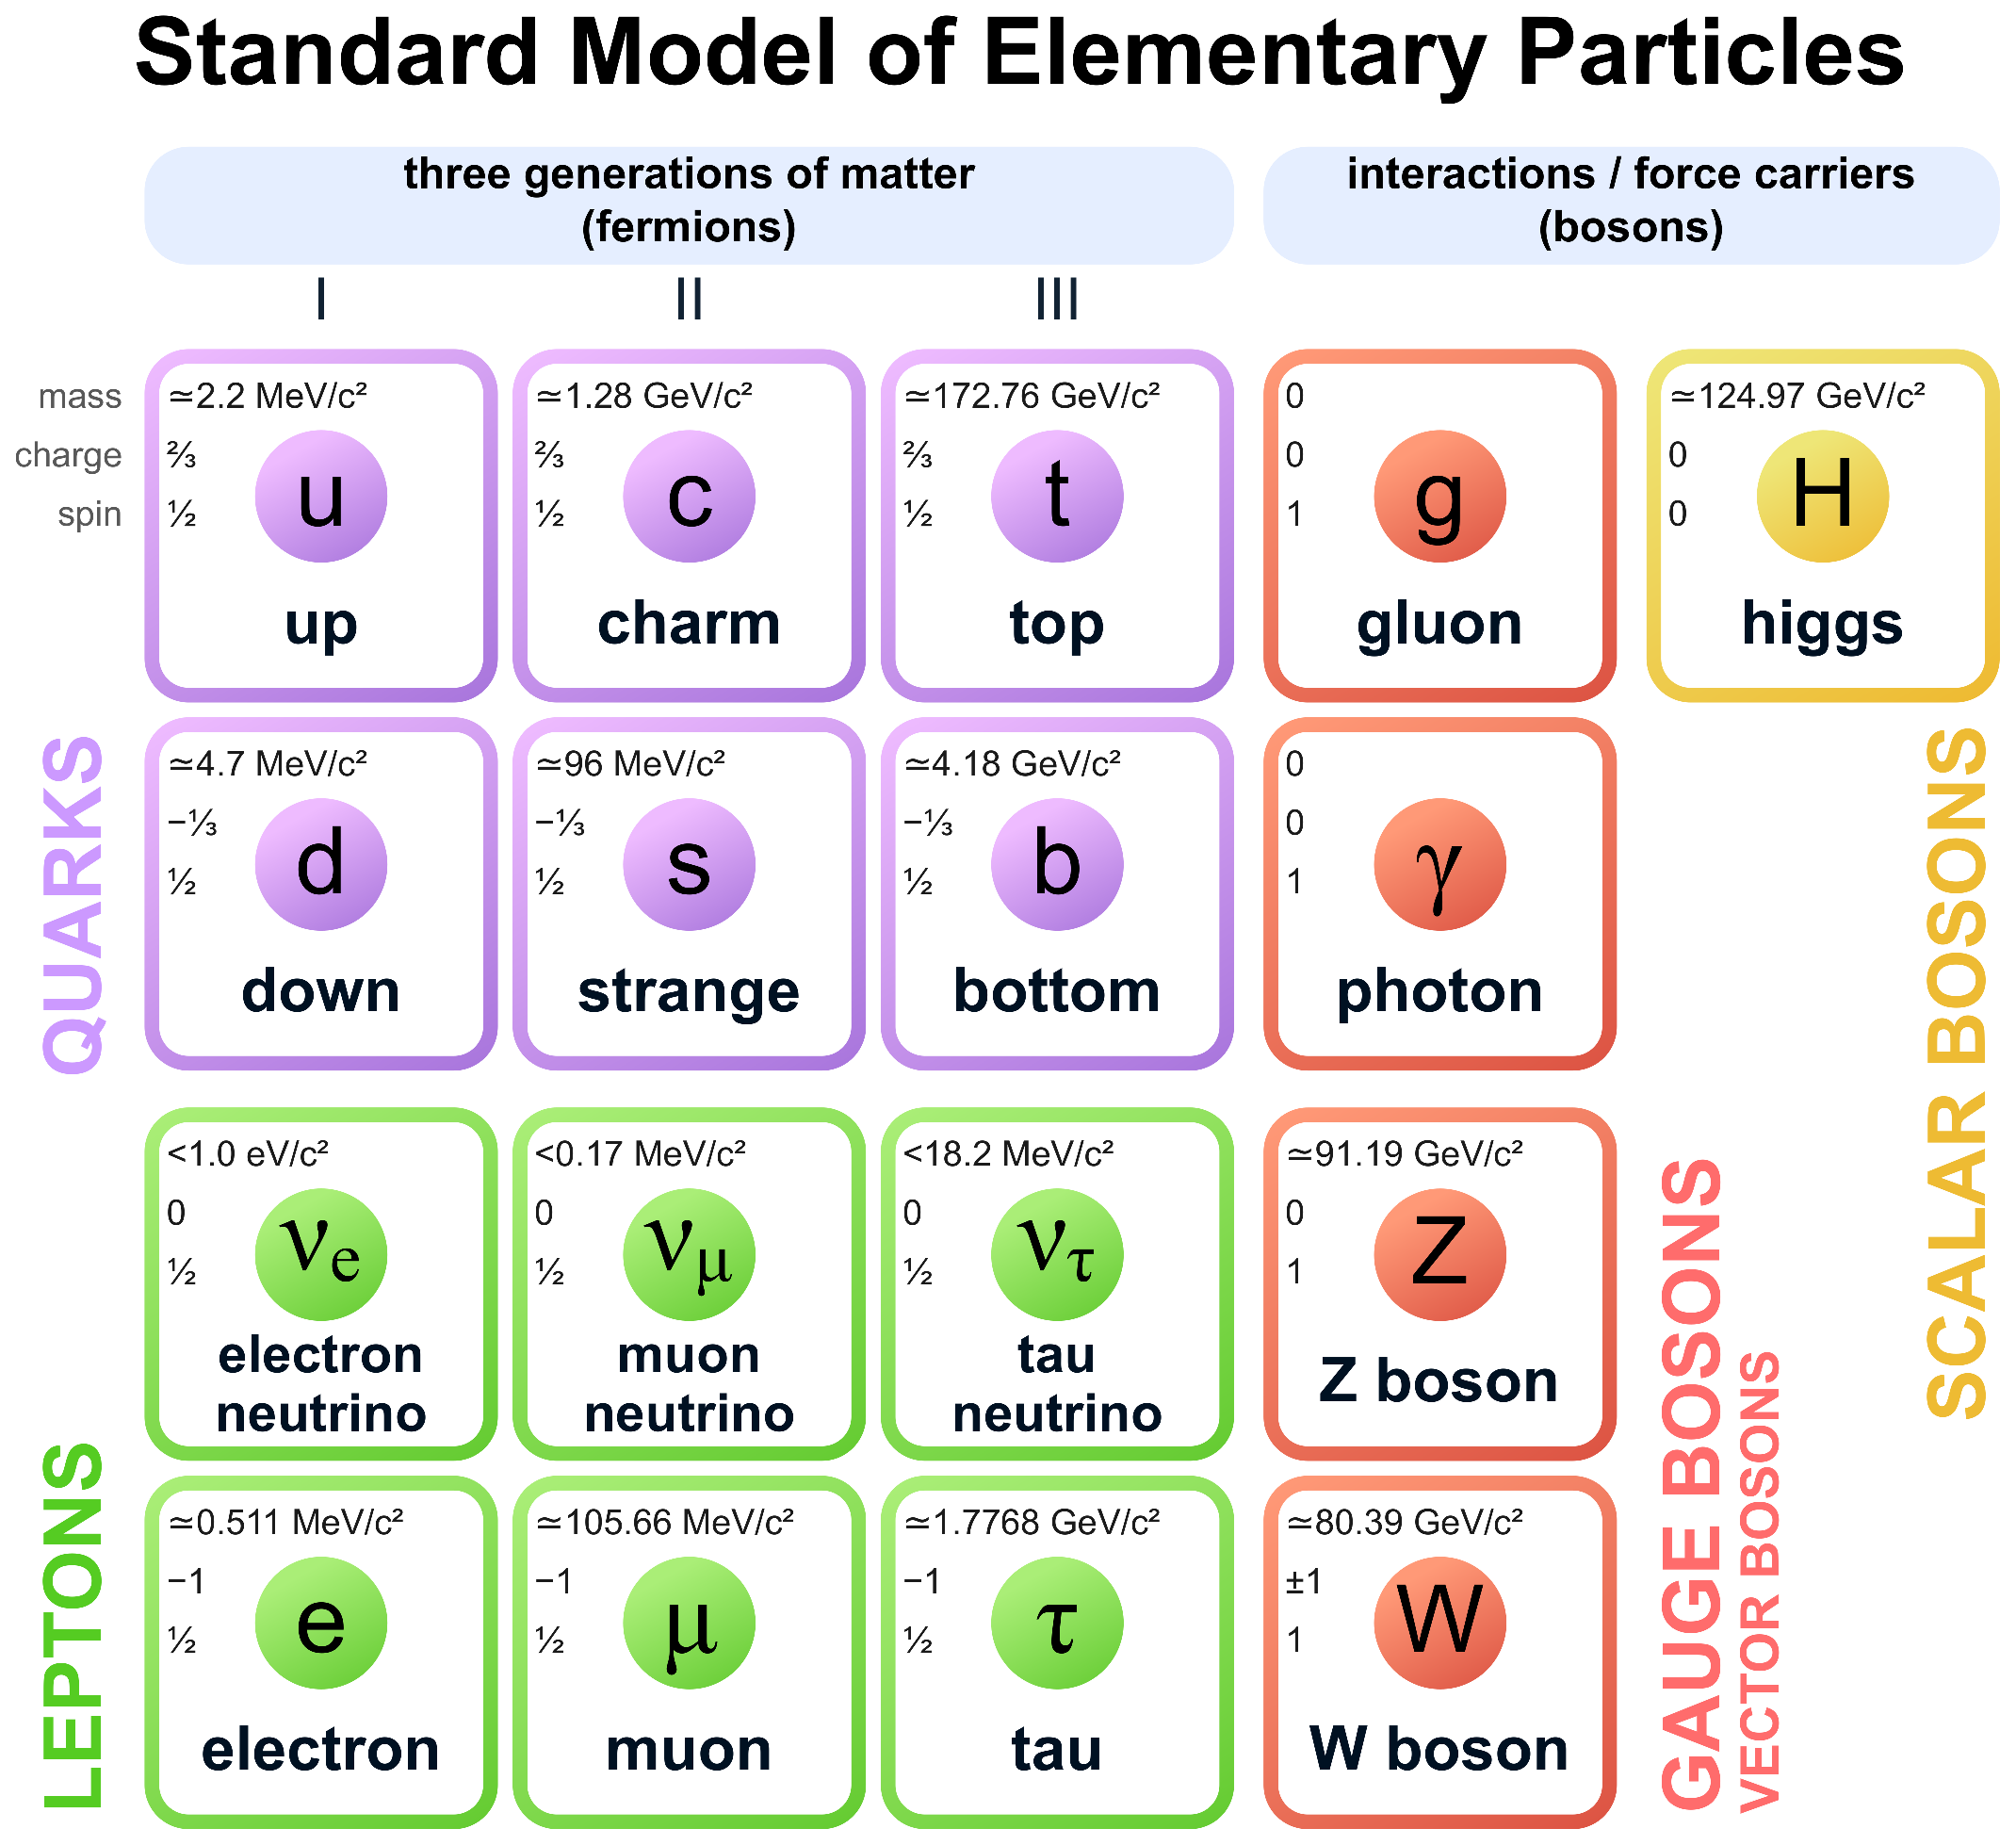
\includegraphics[width=.75\textwidth]{figures/standard_model.eps}
% 	\caption{The elementary particles of the Standard Model subdivided into fermions on the left and bosons on the right. The fermions are further split into quarks at the top and leptons on the bottom, which are each divided into three generations. The bosons are divided into four vector bosons and one scalar boson.}
% 	\label{fig:standard_model}
% \end{figure}

% \section{The Top Quark}
% The top quark ($t$) was discovered in 1995 at \fermilab by the experiments \cdf\cite{top_production01} and \dzero \cite{top_production02}. It is an up-type quark, has a mass of $m_t=172.76\pm0.30,\text{GeV}$, which makes it the heaviest of all known quarks and has a very short lifetime of $\tau_t\approx5\cdot10^{-25}\,\text{s}$ \cite{top_mass}. The \tquark decays via the weak interaction into a \wboson and a down-type quark before it hadronises. The probability of decaying into a certain down-type quark is given by the CKM-matrix \cite{ckm_matrix}. Due to the CKM-matrix having vanishing off-diagonal contributions, \tquarks predominantly decay into \bquarks. The \wboson further decays into a charged lepton and neutrino or into a quark and antiquark so that a variety of signatures as summarised in Tab.~\ref{tab:decay_modes_t} can be measured.

% \begin{table}[t]
% 	\renewcommand{\arraystretch}{1.5}
% 	\centering
% 	\begin{tabular}{R{40mm}C{60mm}C{10mm}C{10mm}}
% 		Signal	& Reaction & Jets & Leptons\\
% 		\hline
% 		Lepton 		& $t\rightarrow bW^+ \rightarrow b(\bar{l}\nu_l)$ & 1 & 1(+1)\\
% 		Jets		& $t\rightarrow bW^+ \rightarrow b(q\bar{q'})$ 	& 3 & 0\\
% 	\end{tabular}
% 	\caption{Possible signals from the \wboson decay modes. The number of leptons in brackets corresponds to the number of neutrinos.}
% 	\label{tab:decay_modes_t}
% \end{table}

% Producing \tquark requires high energies corresponding to the mass of the \tquark. These energies can be achieved in hadrons colliders. Figure~\ref{fig:production_ttz_ttw} shows two example processes for \tquark production in \ttbar-processes. Each of the two \tquarks decays like mentioned before, therefore we get different signals depending on the \wboson decay mode. The possible signals consist either of hadronic decay, leptonic decay or both combined and will be discussed in more detail in Chapter~\ref{ch:methods}. 

% \section{\ttbar{} Production in Association with a $Z$/$W$-Boson}
% When producing \ttbar-pairs, one can also produce additionally a \zwboson. Figure~\ref{fig:production_ttz_ttw} shows example processes for \ttbar-production via gluon-gluon fusion and via quark-antiquark annihilation with an additional \zwboson. A selection of possible signals from \ttbarZ{}/\ttbarW{}-events is summarised in Tab.~\ref{tab:decay_modes_ttz_ttW}.

% The \ttbarZ-events are interesting because they allow studying the coupling of \tquarks to neutral currents of the weak interaction through final state radiation of a \zboson in \ttbar-events. Therefore, \ttbarZ-events allow analysing the third component of the weak isospin of \tquarks.

% The \ttbarW-events are not sensitive to the coupling of \tquarks to charged currents of the weak interaction, because, as seen in Fig~\ref{fig:production_ttz_ttw}, the \wbosons are often emitted as initial state radiation. However, the \ttbarW-processes are sensitive to the initial parton distribution functions (PDF) and thus generate possible constraints onto those PDFs.

% Analysing \ttbarZ/\ttbarW-events together at the same time is particularly interesting because both can generate similar signals and thus are important background processes for each other. Especially studying these events in off-shell regions gives rise to a high rate of background from the respective other process. The kinematic variables, like invariant mass and transverse momentum, of \ttbarW/\ttbarZ off-shell events are also very sensitive to SM-EFT contributions. To be more precise, the sensitivity of SM-EFT contribution increases for higher boson masses \cite{sm_eft_top}.

% \begin{figure}[t]
% 	\centering
% 	\includegraphics[width=.4\textwidth]{figures/ttZ_feynman.png}\hspace{.1\textwidth}
% 	\includegraphics[width=.4\textwidth]{figures/ttW_feynman.png}
% 	\caption{The left Feynman diagram shows an example \ttbarZ-process by gluon fusion. The produced \ttbar-pair emits an additional \zboson. The right Feynman diagram shows a \ttbarW-process by quark-antiquark annihilation.}
% 	\label{fig:production_ttz_ttw}
% \end{figure}

% \begin{table}[t]
% 	\renewcommand{\arraystretch}{1.5}
% 	\centering
% 	\begin{tabular}{R{40mm}L{60mm}C{10mm}C{10mm}}
% 		Signal	& Reaction & Jets & Leptons\\
% 	\hline
% 		\ttbarW-Monoleptonic 	& $t\bar{t}W\rightarrow(bq\bar{q}')(\bar{b}q\bar{q}')(l\bar{\nu_l})$ 				& 6 & 1(+1)\\
% 		\ttbarW-Dileptonic 		& $t\bar{t}W\rightarrow(bq\bar{q}')(\bar{b}l\bar{\nu_l})(l\bar{\nu_l})$ 			& 4 & 2(+2)\\
% 		\ttbarW-Trileptonic 	& $t\bar{t}W\rightarrow(b\bar{l}\nu_l)(\bar{b}l\bar{\nu_l})(l\bar{\nu_l})$ 			& 2 & 3(+3)\\
% 		\ttbarZ-Dileptonic 		& $t\bar{t}Z\rightarrow(bq\bar{q}')(\bar{b}q\bar{q}')(l\bar{l})$ 					& 6 & 2(+0)\\
% 		\ttbarZ-Trileptonic 	& $t\bar{t}Z\rightarrow(bq\bar{q}')(\bar{b}l\bar{\nu_l})(l\bar{l})$ 				& 4 & 3(+1)\\
% 		\ttbarZ-Tetraleptonic 	& $t\bar{t}Z\rightarrow(b\bar{l}\nu_l)(\bar{b}l\bar{\nu_l})(l\bar{l})$ 				& 2 & 4(+2)\\
% 	\end{tabular}
% 	\caption{Possible leptonic signals from \ttbarZ/\ttbarW-events which provides a cleaner measurement. Either \tquark or \zwboson decays into leptons.}
% 	\label{tab:decay_modes_ttz_ttW}
% \end{table}

% \chapter{Experimental Setup}
% For collecting data on the \ttbarW{} and \ttbarZ{} events, one needs to setup a high energy particle collider and an appropriate setup for detecting the corresponding signals.

% The 27\,km long Large Hadron Collider (\lhc) is a proton-proton collider. The centre-of-mass energy reached by the \lhc was around 8\,TeV during Run~I and 13\,TeV during Run~II \cite{lhc1,lhc2}. During Run~III the centre-of-mass energy is expected to reach 14\,TeV \cite{lhc_run3}. Those high-energy collisions produce multiple new particles like \tquarks, which in turn decay into more particles. Detecting events requires a calibrated detector system which measures the properties of the particles such as charge, momentum and energy. Furthermore, reconstructing the events from measured signals requires specific reconstruction algorithms.

% The \atlas-detector \cite{atlas} is a multi-purpose particle detector that consists of different layers for detecting various particles. These layers are built in concentric cylinders around the beam axis. For collecting data on certain events, one must measure the tracks and deposited energies of their decay products. Figure~\ref{fig:atlas} shows a schematic view of those detector layers and each layer is described in the following. 

% \begin{figure}[t]
% 	\centering
% 	\includegraphics[width=.73\textwidth]{figures/atlas.png}
% 	\caption{Cross section of the concentric layers inside the \atlas-Detector.}
% 	\label{fig:atlas}
% \end{figure}

% \paragraph{The Inner Detector:}
% The task of the Inner Detector is to precisely measure the tracks of various charged particles. Because of the 2\,T magnetic field, which is induced by a central solenoid, the moving charged particles are deflected via the Lorentz force. Measurements of the curve radius allows precise measurements of their momentum and reconstructing the particle track. Thus, the tracking system is crucial for $b$-tagging because it makes it possible to identify secondary vertices, which are very good indications for $b$-jets \cite{atlas}. The high density of particles in the detector close to the collision point utilises high-precision measurements using Pixel-, Strip- and Transition Radiation Trackers.

% The Pixel Tracker is the first point of detection and allows tracking near the collision point using small Pixel-modules \cite{atlas}. It is built from silicon to withstand strong radiation from the collision. The semiconductor Strip Tracker (SCT) consists of longer strips that also contribute to the tracking by offering larger scale measurement.

% The Transition Radiation Tracker (TRT) is built from thin and long polyimide straws \cite{atlas}. These straw tubes are filled with a gas mixture  and while they offer a worse resolution, they allow for a relatively cheap way to cover a greater volume and hence, contribute to a precise measurement.

% \paragraph{The Calorimeters:}
% As seen in Fig.~\ref{fig:atlas}, the calorimeters are built around the Inner Detector and the solenoid magnet. In general, the calorimeters measure the energy of particles by stopping them. The calorimeter system used in the \atlas-detector is subdivided into the electromagnetic and the hadronic calorimeter. Both are sampling calorimeters that have an absorber material, which induces particle showers and an active medium, which is used for measuring the signals \cite{atlas_calorimeter}.

% The electromagnetic calorimeter measures all particles that interact electromagnetically. Those charged particles and photons each create an electromagnetic shower which can be used to reconstruct the initial particles. It offers a precise measurement of the deposited energy and the location of the energy-deposition. It is built from Lead as the absorber and liquid Argon as active medium \cite{atlas_calorimeter}.

% The hadronic calorimeter absorbs particles that pass the electromagnetic calorimeter and interact via the strong force. The hadronic showers created can produce additional electromagnetic sub-showers which makes them more difficult to reconstruct and less precise. Its absorber material is Copper and its active material is also liquid Argon \cite{atlas_calorimeter}.

% \paragraph{The Muon Spectrometer:}
% The Muon Spectrometer is the outermost layer and follows a similar approach as the Inner Detector to measure the momentum of muons by tracking their deflected trajectory. The magnetic field responsible for the deflection is generated by outer toroidal magnets. Data on muons can be important for analysing neutrino-related events.

% \chapter{Methods}
% \label{ch:methods}
% As mentioned above, there are different signal channels for \ttbarZ/\ttbarW-processes which can be used for measuring these events. Each signal channel has certain advantages and disadvantages for an analysis as described in the following.

% \paragraph{Full Hadronic:} 
% Full hadronic decays have high branching ratio ($\sim45\%$ for \ttbar-production) but they are difficult to reconstruct because of their produced jets. In theory, the measured final particles just have to collected into cone-formed jets to reconstruct the initial particles through conservation laws, however, there are multiple challenges to this. Missed information because of energy leakage or absorber material losses as well as electronic noise, jet overlapping and limited algorithm efficiencies makes reconstructing the initial state difficult. This decay mode produces 3 jets per \tquark, of which at least one is expected to be a $b$-jet, and two jets from bosons.
 
% \paragraph{Full Leptonic:}
% Full leptonic decays are rarer ($\sim10\%$ for \ttbar-production) but cleaner measurements of lepton signals. These leptonic decays refer to electrons and muons only, because tau-leptons decay into hadrons and thus create jets, making them more difficult to reconstruct. Their signal is cleaner, because they do not form hadron-jets but smaller electromagnetic showers in the calorimeter. However, the produced neutrinos can not be measured, their energy has to be measured indirectly via the missing energy of the process. This decay mode produces only 1 $b$-jet per \tquark.

% \paragraph{Semi-Leptonic:}
% There are also some semi-leptonic channels which consist of some particles decay hadronically and some leptonically. Those also have a high branching ratio ($\sim45\%$ for \ttbar-production) and offer a cleaner measurement than full hadronic channels, because of less jets per event. But the jet reconstruction makes calculating the missing energy of the involved neutrinos more difficult. The number of jets depends on the exact decay of each particle but there is at least 1 $b$-jet per \tquark and there can not be more jets than in a full hadronic decay.

% \section{Comparison to Previous Studies}
% This thesis will focus on the trileptonic decay channel of \ttbarZ/\ttbarW, which is a semi-leptonic decay and is presented in Tab.~\ref{tab:decay_modes_ttz_ttW}. The current analysis can use larger datasets like the full Run~II dataset, collected during the years 2015-2018. To identify the trileptonic channel, certain signal regions have to be defined. These are characterised by the number of measured leptons, jets and identified b-jets as well as momentum and sum of charge of the leptons.

% In previous studies \cite{atlas_ttw_ttz,atlas_ttz}, jets were reconstructed using the anti-$k_t$ algorithm \cite{anti_k_algorithm} and $b$-tagging was performed by using the mv2c10-algorithm \cite{b_tagging}. Current analysis uses the same parameters for jet-object reconstruction but uses the newer DL1r-algorithm \cite{dl1r_algorithm}, which is based on neural networks and has an improved performance compared to the mv2c10-algorithm. 

% Moreover, current research uses some new multivariate analysis (MVA) methods for the (semi-)leptonic channels. These also allow for analysis of the off-shell \zboson processes which will be conducted in this analysis. The isolation of lepton object definitions were previously done using the FCTight-algorithm \cite{fctigth_algorithm}, the current analysis uses the PLVLoose-algorithm \cite{plvloose_algorithm}.

% This analysis will also utilise up-to-date recommendations of the combined performance groups within ATLAS \cite{cp_group_ttbar} to further decrease systematic uncertainties in comparison to previous studies. Additionally, precision measurements and better understanding of background signals, especially events with misidentified or non-prompt leptons \cite{atlas_ttw_ttz} for trileptonic decays, allow for reduced modelling uncertainties.


% \chapter{Timetable}
% For a structured schedule, the 14-week period of working on the Bachelor Thesis is divided into different tasks for each week. The general timetable is shown in Tab.~\ref{tab:timetable}.
% \begin{table}[ht]
% 	\renewcommand{\arraystretch}{1.5}
% 	\centering
% 	\begin{tabular}{l|p{12cm}}
% 		Week	& Task\\
% 		\hline
% 		1 		& Research previous \ttbarZ/\ttbarW analysis \\
% 		2		& Study analysis framework (TRExFitter, MVA-Trainer)\\
% 		3-5 	& Construction of signal- and background-framework for \ttbarZ/\ttbarW analysis including different fits\\
% 		6		& Implementation of systematic uncertainties\\
% 		7-8		& Investigation of EFT-sensitive variables in signal region\\
% 		9-11	& Improvement of signal region through MVA-methods and neural networks\\
% 		12-14	& Writing bachelor thesis\\
% 	\end{tabular}
% 	\caption{The table summarises the weekly schedule for the time required to complete the bachelor's thesis.}
% 	\label{tab:timetable}
% \end{table} 


%\appendix
%\chapter{erster Anhang}
%Text\dots
%\chapter{zweiter Anhang}
%Text\dots

\bibliography{datenbank} 

%\begin{otherlanguage}{ngerman}
%\Declaration
%\end{otherlanguage}

\end{document}
